\documentclass{article}
\usepackage[T1]{fontenc}
\usepackage[utf8]{inputenc}
\usepackage[portuguese]{babel}

\title{Lista 4 \\
\large Introdução à Análise Numérica \\
Solução numérica de EDOs}
\author{Lucas Emanuel Resck Domingues}
\date{\today}

\usepackage{natbib}
\usepackage{graphicx}
\usepackage{amsmath}
\usepackage{listings}
\usepackage{multirow}
\usepackage{hyperref}
\usepackage{amsfonts}

% \lstset{columns=fullflexible}

% Hyperlinks
\usepackage{hyperref}
\hypersetup{
    colorlinks=true,
    allcolors=,  % Nothing change colors
    urlcolor=blue  % URL changes color
}

\begin{document}

    \maketitle

    \begin{enumerate}
        \item[4.]
            \begin{enumerate}
                \item A função que constrói uma aproximação
                    da solução utilizando do método Forward
                    Euler foi implementada e pode ser vista
                    no Apêndice \ref{appendix:forward_euler}.

                    O intervalo de integração é particionado
                    em $N$ intervalos de comprimento igual a $h$,
                    e o método é calculado em cada ponto da partição
                    utilizando o método Forward Euler. Ao final,
                    um gráfico do valor exato e do valor aproximado
                    da função no intervalo especificado é exibido.

                \item As Figuras \ref{fig:forward_1},
                    \ref{fig:forward_2} e \ref{fig:forward_3}
                    exibem os resultados da aproximação para diferentes
                    valores de $h$, com intervalo de integração $[0, 1]$
                    e condição inicial $x(0) = \{1, 1\}$. Nas Figuras,
                    também vamos os erros na norma infinito (entre
                    aproximação e valor exato), além de uma comparação
                    no gráfico. Observamos que a solução para a segunda
                    coordenada, $x_2$, sempre fica boa, enquanto a solução
                    para $x_1$ só fica boa para $h < 0.002$.
                
                \begin{figure}[!h]
                    \centering
                    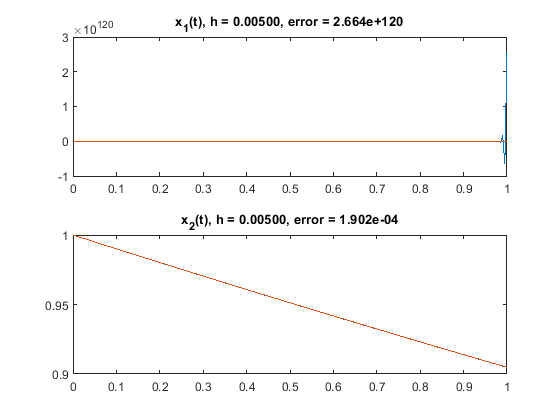
\includegraphics[width=\textwidth]{forward_1.png}
                    \caption{Aproximação pelo método (em azul) e
                    solução exata (em laranja), para $h = 0.005$,
                    no intervalo $[0, 1]$, com $x(0) = \{1, 1\}$.
                    O erro calculado é a norma infinito entre as
                    soluções. Vemos que a solução para a segunda
                    coordenada, $x_2$, ficou boa, porém para a primeira
                    coordenada, $x_1$, ficou péssima.}
                    \label{fig:forward_1}
                \end{figure}
                
                \begin{figure}[!h]
                    \centering
                    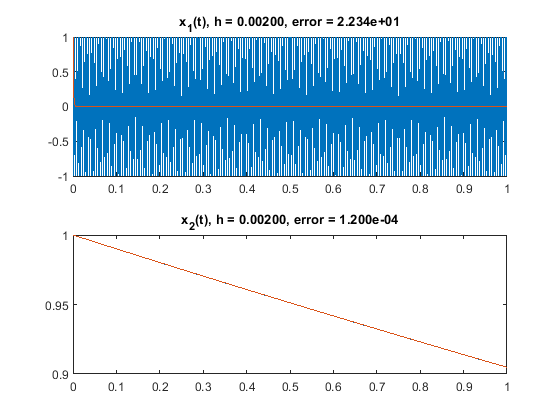
\includegraphics[width=\textwidth]{forward_2.png}
                    \caption{Aproximação pelo método (em azul) e
                    solução exata (em laranja), para $h = 0.002$,
                    no intervalo $[0, 1]$, com $x(0) = \{1, 1\}$.
                    Vemos que a solução para a segunda
                    coordenada, $x_2$, ficou boa, porém para a primeira
                    coordenada, $x_1$, ficou péssima.}
                    \label{fig:forward_2}
                \end{figure}
                
                \begin{figure}[!h]
                    \centering
                    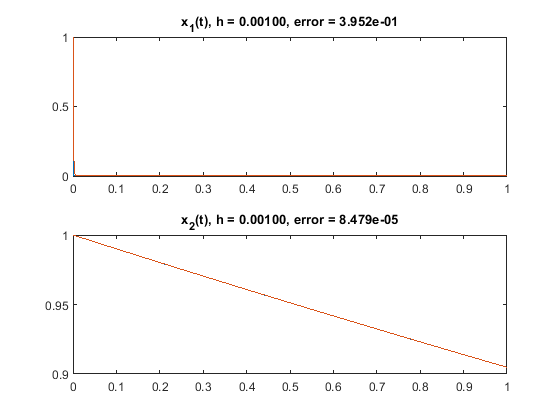
\includegraphics[width=\textwidth]{forward_3.png}
                    \caption{Aproximação pelo método (em azul) e
                    solução exata (em laranja), para $h = 0.001$,
                    no intervalo $[0, 1]$, com $x(0) = \{1, 1\}$.
                    Vemos que a solução para a segunda
                    coordenada, $x_2$, ficou boa, assim como para a primeira
                    coordenada, $x_1$.}
                    \label{fig:forward_3}
                \end{figure}
            \end{enumerate} 
    \end{enumerate}

    \clearpage

    \appendix

    \section{Forward Euler}
        \label{appendix:forward_euler}

        \begin{lstlisting}[language=Matlab]
            TO-DO
        \end{lstlisting}

\end{document}
